\section{Nombre de Clusters}
L'analyse hiérarchique va nous permettre de déterminer le nombre de cluster que nous pouvons envisager. Pour ce faire nous utilisons le composant Hierarchical Clustering de Knime avec comme configuration Linkage type : SINGLE.

\subsection{Santé}
Nous réalisons le Hierarchical Clustering avec les attributs santé. Cependant nous décidons d'enlever l'attribut population total car c'est une valeur brute, elle fausse le clustering. Nous obtenons le graphe des distances suivant : 

\begin{figure}[H]
	\begin{center}
		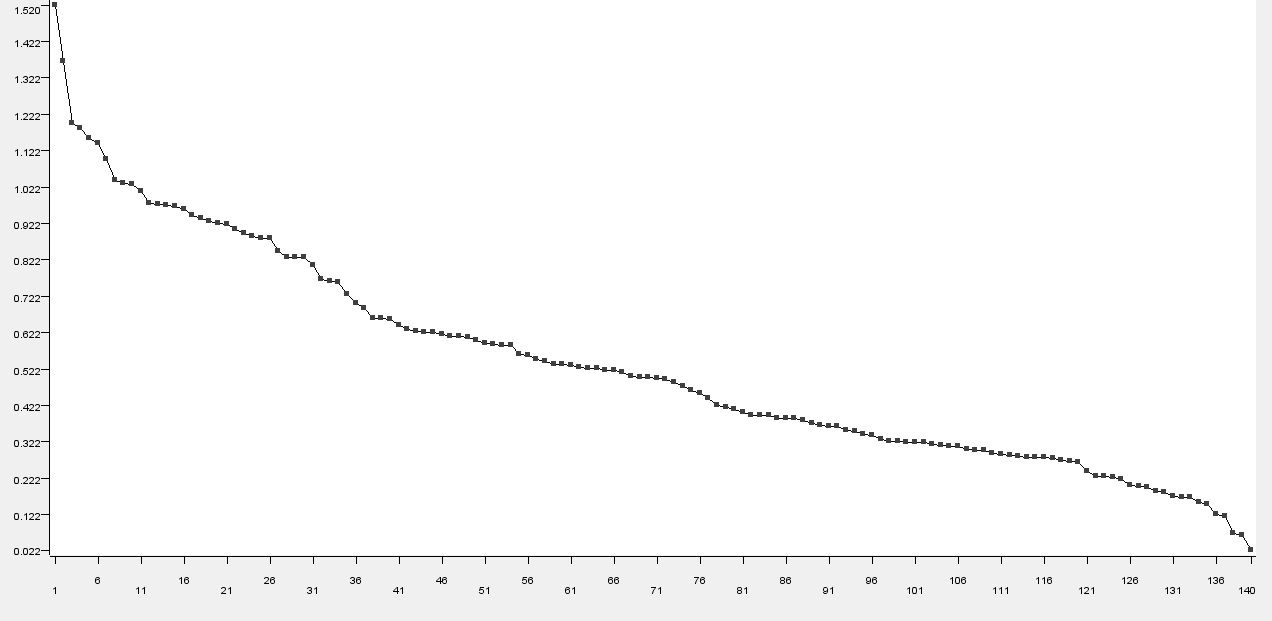
\includegraphics[scale=0.5]{Image/DistanceSanteNoMissing2}
		\caption{Graphe de distance de l'indicateur Santé \jeuc}
	\end{center}
\end{figure}

Suite à l'analyse de ce graphe nous décidons de faire 3 Clusters.

\subsection{Politique économique}
Nous réalisons la même démarche que précédemment mais avec les attributs de l'indicateur Politique économique. Nous obtenons le graphe de distance suivant : 
\begin{figure}[H]
	\begin{center}
		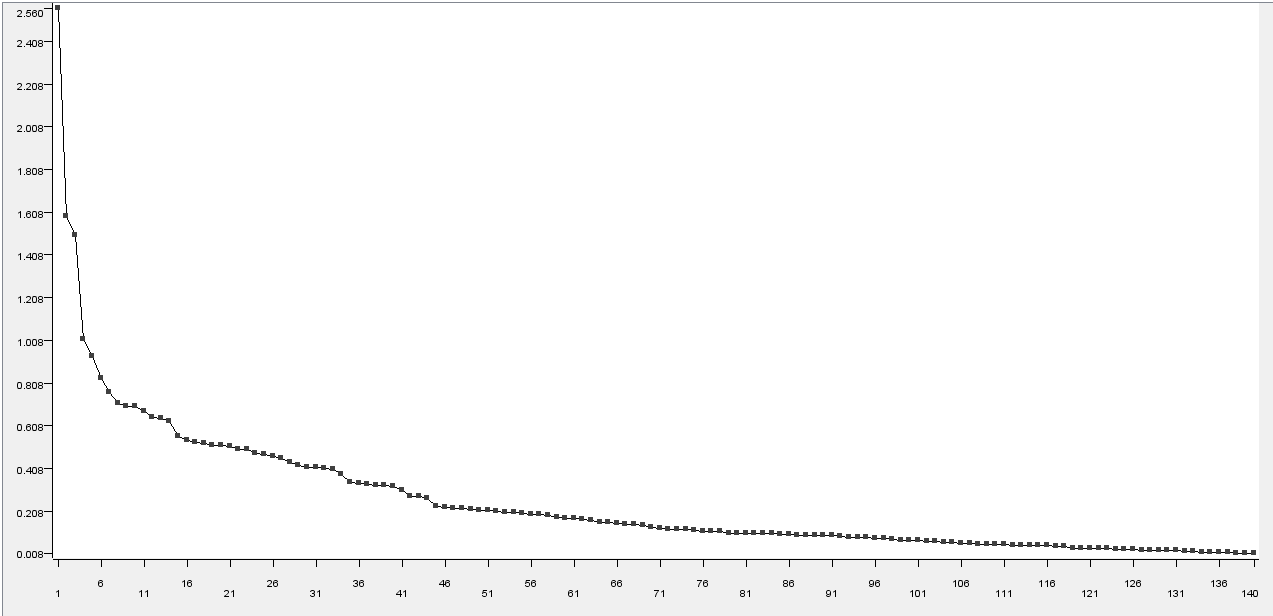
\includegraphics[scale=0.5]{Image/DistancePolitiqueNoMissing2}
		\caption{Graphe de distance de l'indicateur Politique économique\jeuc}
	\end{center}
\end{figure}

Après étude du graphe nous ferons 4 clusters.